\chapter{Techniques informatiques} % (fold)
\label{cha:techniques_informatiques}

Dans ce chapitre, je vais parle des outils et des techniques utilisés pendant ce stage. Ces outils contient les outils utilisé dans l'équipe pour le but de mieux communiquer et mieux collaborer. Il y a des outils utilisé pour développement, y compris l'IDE, les outils pour débug et amélioration etc. Sauf-ci, je vais quand même présenter les frameworks, conception utilisé pour ce projet.

\section{Outils de Collaboration} % (fold)
\label{sec:outils_de_collaboration}

Pendant ce stage, j'ai touché plusieurs techniques nouvelles, appris beaucoup des façons à développement. Sauf ci, j'ai appris beaucoup des outils de collaborations, et apprendre la façon de travaille en équipe. Dans ce section, je vais parler des outils de collaborations

\subsection{Producteev et Redmine} % (fold)
\label{ssub:producteev_et_redmine}

La raison de mettre les 2 outils ensemble est non seulement les 2 outils se ressemblent, mais aussi, ils sont les plus importantes. Au début de stage, dans un première temps, ce que j'ai touché est le Producteev. Producteev est utilisé par Chugulu Games pendant certaines années. Cet été, ils ont décidé de changé à utiliser un autre outil qui s'appelle Redmine. 

\subsubsection{Producteev} % (fold)
\label{ssub:producteev}


\begin{figure}[htbp]
	\centering
		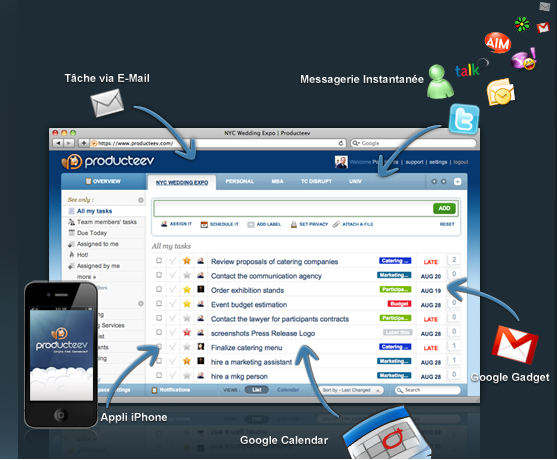
\includegraphics[width=6in]{Image/Producteev.png}
	\caption{caption}
	\label{fig:Image_Producteev}
\end{figure}

Producteev est un gestionnaire de tâches à la fois B2B et B2C dont l’ADN est collaboratif. D’une utilisation personnelle à un nombre de connectés illimités en entreprise, la solution fonctionne online et offline en interface avec les comptes e-mail, Facebook ou Google Calendar entre autres dans des versions web et mobiles. Il a ces fonctionnalités :
\begin{description}
	\item[Gestion de plusieurs équipes] Gérer plusieurs équipes grâce à Producteev en utilisant les fonctionnalités simples intégrées. Inviter les membres des équipes, ajustez les paramètres de confidentialité et bien plus encore pour votre liste de tâches.
	\item[Filtres et rapports] Générer facilement des rapports sur le projet et sur l'activité d'équipe. Par exemple, recevoir toutes les semaines un email d'aperçu des avancées d'équipe.
	\item[Emails récapitulatifs] Recevez chaque jour le rapport journalier/hebdomadaire, pour avoir un aperçu de l'équipe.
	\item[Tâches prioritaires]  L'algorithme utilisé pour la gestion des tâches prioritaires trie automatiquement les tâches et  suggère à faire ensuite
	\item[Synchroniser vos tâches avec Google Agenda] Synchronisez Producteev avec Google Agenda ou placer-y simplement une tâche à la fois. 
\end{description}

Sauf ces fonctionnalité, producteev est possible de synchroniser avec ses logiciel client sous Mac ou iPhone, avec Google. Et, il est possible de se communiquer en utilisant les mails. Envoyer et recevoir les nouvelles par les mails. 

% subsubsection producteev (end)

\subsubsection{Redmine} % (fold)
\label{ssub:redmine}

% TODO add the logo redmine

Redmine est une application web Open Source de gestion complète de projet en mode web, développé en Ruby sur la base du framework Ruby on Rails.
Il a été créé par Jean-Philippe Lang. D'autres développeurs venant de la communauté des utilisateurs de Redmine contribuent depuis au projet. Il utilise la syntaxe Textile pour ses pages de wiki et de nombreux autres emplacements où l'utilisateur peut entrer du texte : 
\begin{itemize}
	\item descriptif de bogue ou de demande, ainsi que les commentaires associés
	\item forums
	\item nouvelles
	\item description
\end{itemize}

La fonctionnalité de Redmine comporte la liste suivante:
\begin{itemize}
	\item gestion multi-projets
	\item gestion fine des droits utilisateurs définis par des rôles
	\item gestion de groupes d'utilisateurs
	\item rapports de bogues (bugs), demandes d'évolutions
	\item Wiki multi-projets
	\item forums multi-projets
	\item news accessibles par RSS / ATOM
	\item notifications par courriel (mail)
	\item gestion de feuilles de route, GANTT, calendrier
	\item historique
	\item intégration avec divers suivis de versions : SVN, CVS, Mercurial, Git, Bazaar \& Darcs
	\item identification possible via LDAP
	\item multilingue (25 langues disponibles pour la 0.7.0)
	\item support de plusieurs bases de données : MySQL, PostgreSQL ou SQLite
\end{itemize}

Par rapport au Producteev, redmine a des avantages evident. La plus importante est que redmine est gratuit. Il est possible d'installer redmine dans le site web interne d'entreprise. Il a un système de notification mieux que producteev. Redmine supporte beaucoup de personnalisation. Il permet de personnalisé les couleur, les interfaces etc. De plus, redmine supporte 30+ de language. 

Pendant ce stage à chugulu, nous avons utilisé beaucoup cet outil pour se communiquer, mettre à jours nos statues. Il est aussi facile pour le chef de projet, pour mon encadrant de reporter les nouvelles issus, de contrôle les progrès des tâches assigné à chaque développeur. L'interface de redmine est beaucoup mieux par rapport à l'interface de producteev. Sur redmine, nous pouvons mettre à jours nos tâches et nos statues simplement par cliquer à droit sur la souris. 

Un autre avantage important est qu'il peut être installé à interne de l'entreprise. C'est beaucoup mieux par rapport à un site web comme Producteev. Non seulement la niveau de sécurité, mais aussi que on peut maintenir nous même. Si un jour, Producteev est disparu, nous allons perdre tous nos informations.

% subsubsection redmine (end)

% subsubsection producteev_et_redmine (end)

\subsection{Git \& Github} % (fold)

\subsubsection{Git} % (fold)


\begin{figure}[htbp]
	\centering
		
\includegraphics[width=6in]{Image/GitLogo.png}
	\caption{caption}
	\label{fig:Image_GitLogo}
\end{figure}

Git est un logiciel de gestion de versions décentralisée. C'est un logiciel libre créé par Linus Torvalds, le créateur du noyau Linux, et distribué sous la GNU GPL version 2. Il est crée par Linus Torvalds, qui est aussi le créateur de Linux. Git ne repose pas sur un serveur centralisé. C'est un outil bas niveau, qui se veut simple et très performant, dont la principale tâche est de gérer l'évolution du contenu d'une arborescence. Chaque répertoire git contient une base des données local, y contient toutes les fichiers, les commits, les traces, les branches etc. Il est encore un avantage par rapport aux autre logiciel version contrôle comme SVN, c'est que git nous permet de choisi un ou plusieurs fichier. 

Git possède deux structures de données : une base d'objets et un cache de répertoires. Il existe quatre types d'objets :

\begin{itemize}
	\item l'objet blob, qui représente le contenu d'un fichier (l'origine de cette dénomination est probablement à chercher dans les Binary Large OBjects des bases de données).
	\item l'objet tree ("arbre" en anglais), qui est une liste d'objets de type blobs et des informations associées à chaque blob, tel que le nom du fichier et les permissions. Cet objet décrit l'arborescence des sources à un temps donné.
	\item l'objet commit, qui donne accès à l'historique d'une arborescence de source. Il contient un message de log, un objet arbre et pointe vers un ou plusieurs objets commit parents.
	\item l'objet tag qui est une manière de représenter un commit spécifique. Il est en général utilisé pour marquer certains commits, par exemple par un numéro ou un nom de version (2.1 ou bien Hardy Heron).
\end{itemize}

La base des objets peut contenir n'importe quel type d'objets. Une couche intermédiaire, utilisant des index (les sommes de contrôle), établit un lien entre les objets de la base et l'arborescence des fichiers.
Chaque objet est identifié par une somme de contrôle SHA-1 de son contenu. Git calcule la somme de contrôle et utilise cette valeur pour déterminer le nom de fichier de l'objet. L'objet est placé dans un répertoire dont le nom correspond aux deux premières lettres de la somme de contrôle. Le reste de la somme de contrôle constitue alors le nom du fichier pour cet objet.

Git enregistre chaque révision dans un fichier en tant qu'objet blob unique. Les relations entre les objets blobs sont déterminées en examinant les objets commit. En général, les objets blobs sont stockés dans leur intégralité en utilisant la compression de la zlib. Ce principe peut rapidement consommer une grande quantité de place disque ; de ce fait, les objets peuvent être combinés dans des archives, qui utilisent la compression différentielle (c'est-à-dire que les blobs sont enregistrés sous la forme de différences par rapport aux autres blobs).
% subsubsection Git (end)

\subsubsection{Github} % (fold)


\begin{figure}[htbp]
	\centering
		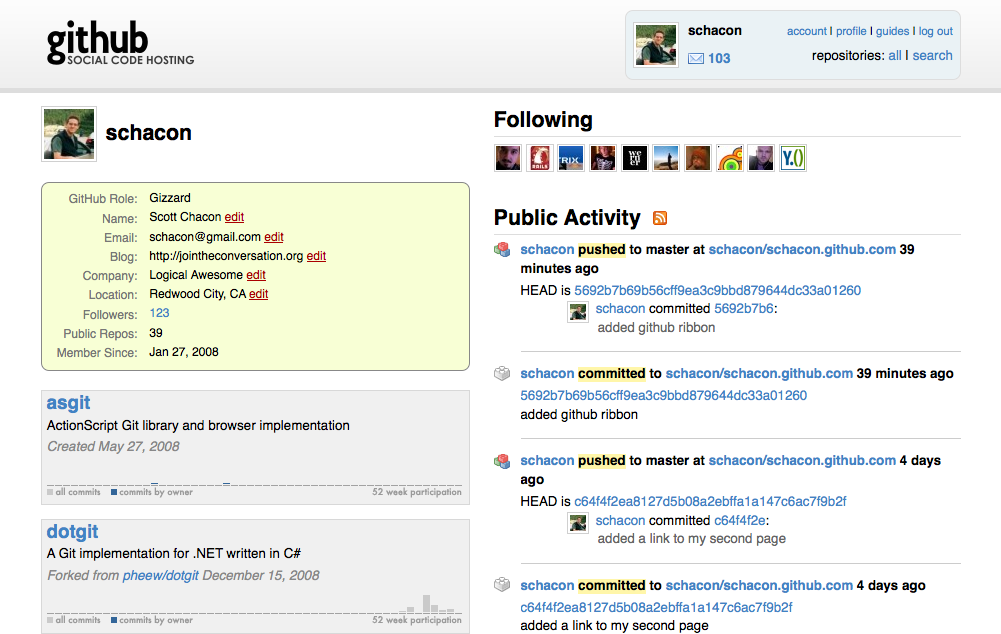
\includegraphics[width=6in]{Image/githubCapture.png}
	\caption{caption}
	\label{fig:Image_githubCapture}
\end{figure}


GitHub est un service web d'hébergement et de gestion de développement de logiciels, utilisant le programme Git. Ce site est développé en Ruby on Rails. GitHub propose des comptes professionnels payants, ainsi que des comptes gratuits pour les projets open source. Il est le meilleur site web du monde pour utiliser git. Github supporte la collaboration. Il supporte le fonction de folk. Nous pouvons faire une copie de n'importe quel projet qui nous intéresse. Github supporte plusieurs type de management. Par défaut, nous pouvons avoir une répertoire gratuits, mais tous nos fichiers sont publié. Github fournit quelque options pour les utilisateurs d'entreprise. Par exemple, nous pouvons payer 7 dollar par mois, et obtenons 5 repositoir avec 1 collaborateur, qui peut avoir 0.6GB d'espace. 

Github travaille mieux par rapport aux serveur de svn chez Chugulu Game. Chugulu games a commencé à utiliser git \& github cet été. Il devient mieux par rapport avant.
% subsubsection Github (end)

% subsection Git \& Github (end)

\subsection{XMind} % (fold)


\begin{figure}[htbp]
	\centering
		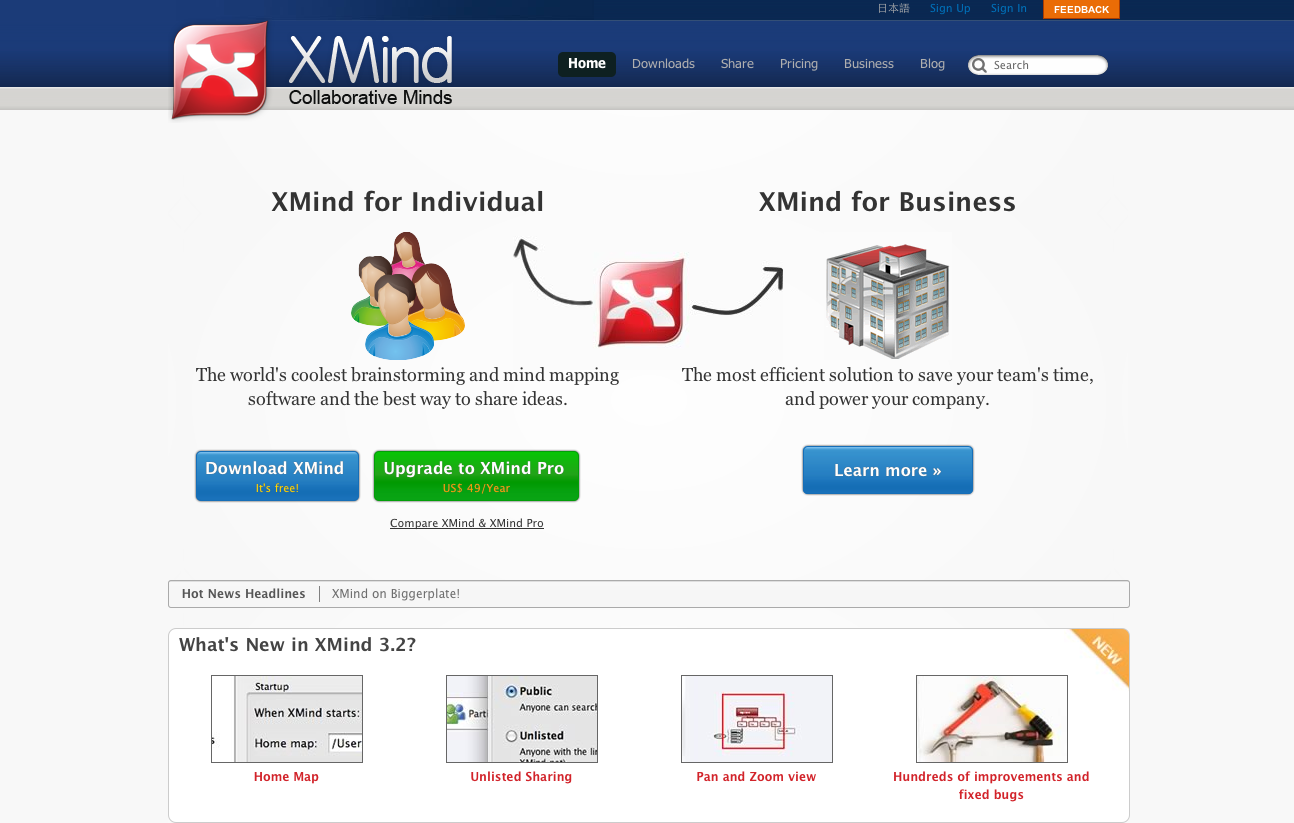
\includegraphics[width=6in]{Image/Xmind.png}
	\caption{caption}
	\label{fig:Image_Xmind}
\end{figure}

XMind est un outil très pratique. Chugulu game utilise cet outil beaucoup pour organiser les idées, présenter les schémas. 

XMind est un logiciel Open Source, pour brainstorming. Il a deux version, une version gratuit et une version plus puissante mais payante. XMind est basé sur Eclipse, qui fournit l'assistance aux utilisateurs de trouver ses idées, organiser différente type des schémas, partager avec leur collaborateurs. Il supporte Mind Map, Ishikawa diagrams (fishbone diagrams ou cause-and-effect diagrams), tree diagrams, organization charts, et spreadsheets. Il est possible de l'utiliser pour manager les savoir-faire, les notes des conférences, et GTD. 

La version payante supporte exporter les mind map en format Microsoft Word, Power point, PDF etc.

Pendant ce stage, j'ai utilisé XMind pour organiser mes idées, construire les schéma nécessaire, et les a inséré dans les documents internes. En utilisant XMind, j'ai gagné beaucoup de temps. C'est aussi important et facile pour moi de mieux présenter mes idées.

% subsection XMind (end)
% section outils_de_collaboration (end)

\section{Outils de Développement} % (fold)
\label{sec:outils_de_développement}

\subsection{XCode} % (fold)
\label{sub:xcode}

% TODO add logo xcode
\begin{figure}[htbp]
	\centering
		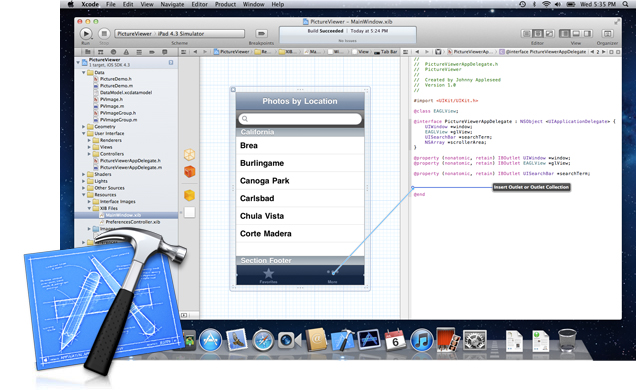
\includegraphics[width=6in]{Image/tools_overview_xcode_20110711.jpg}
	\caption{caption}
	\label{fig:Image_tools_overview_xcode_20110711}
\end{figure}

XCode est un environnement de développement pour MacOS. Il est crée par l'entreprise Apple, et utilisé seulement sous MacOX. XCode est un IDE très puissante. Il comporte presque toute les caractéristiques commune des IDE, sauf ci, il supporte des techniques spécial pour améliorer la productivité sous MacOS. XCode supporte plusieurs langage, y compris C, C++, Objective C, PHP, Ruby, etc.. XCode fournit une interface unifié, respecter le standard d'interface de MacOS. Il est très facile à apprendre pour un utilisateur de MacOS. Surtout XCode 4, il fournit une interface comme iTunes. Fourni avec toute une suite logicielle (graphiques, audio, etc.) pour développeurs et programmeurs, il permet de créer des logiciels utilisant toutes les fonctionnalités, la puissance et la stabilité de Mac OS X et d'UNIX. Par rapport aux Visual Studio de Microsoft, cet IDE est gratuit.

Maintenant, la nouvelle version est XCode 4.1. 

Le raison pour choisir XCode comme l'IDE principale est évident. Parce que, il est la seule choix pour développer l'application sur iOS. Il supporte les plus de fonctionnalité, les outils pour développer. Il est aussi désigné et amélioré spécialement pour iOS développé. Il n'as pas de raison pour ne pas utiliser ce produit.

% subsection xcode (end)

\subsection{Instruments} % (fold)
\label{sub:instrument}

\begin{figure}[htbp]
	\centering
		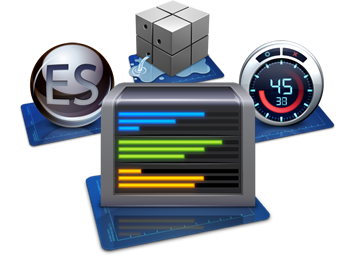
\includegraphics[width=6in]{Image/instrumentslogo.jpg}
	\caption{caption}
	\label{fig:Image_instrumentslogo}
\end{figure}

Instruments est un logiciel crée par Apple. Il est un outil hyper fort. Instrument est un logiciel pour développeur de tracer et profiling le projet MacOS et iOS dynamiquement. Il est très pratique pour débugger, résoudre le performance d'application. Il est aussi très utile pour améliorer le performance. Pendant ce stage, j'ai utilisé cet outil pour améliorer la performance de <<Playboy-Spot>>. 
Voici une capture de l'écran quand j'ai fait tracer tous les threads pendant l'exécution. 

% TODO add instrument capture d'écran

\begin{figure}[htbp]
	\centering
		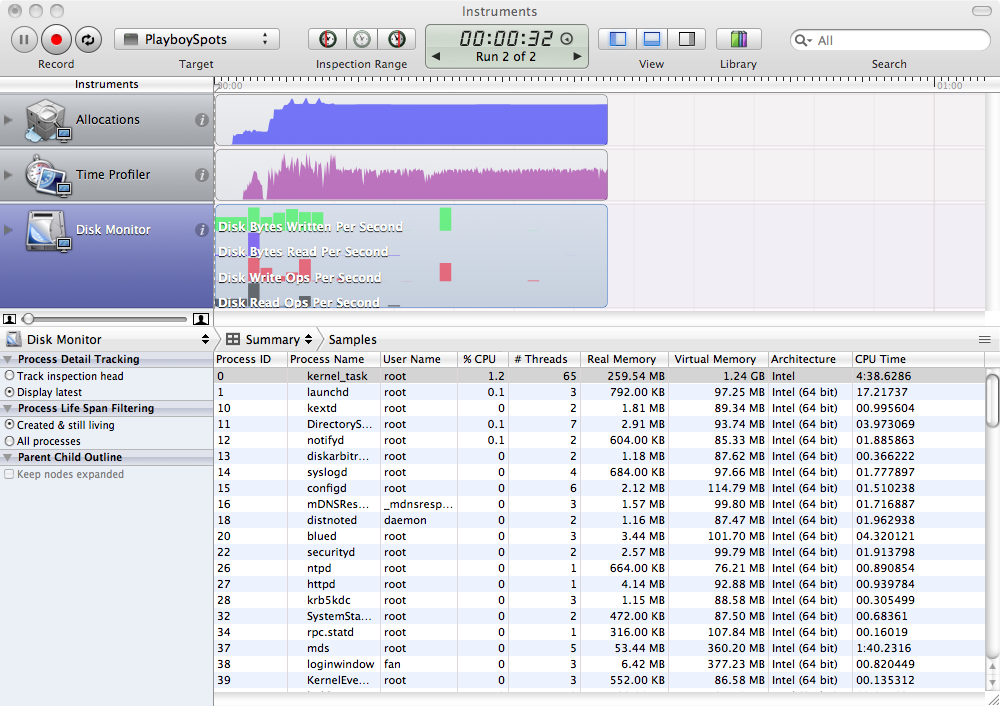
\includegraphics[width=6in]{Image/captureInstruments.png}
	\caption{caption}
	\label{fig:Image_captureInstruments}
\end{figure}

% subsection instrument (end)

% section outils_de_développement (end)

\section{Technique utilisé} % (fold)
\label{sec:technique_utilisé}

% section technique_utilisé (end)


% chapter techniques_informatiques (end)